






%------------------------------------------------------------------------------
%
%	BA6 - Database systems
%
%	Authors :
%		203267 - Bastien Antoine
%		183785 - Denoréaz Thomas
%		185078 - Dieulivol David
%
%	Versions :
%		2013.03.30 - Initial version
%

%--------------DOCUMENT--------------------------------------------------------
\documentclass[a4paper,oneside,11pt]{article}  % Type de document
\usepackage[french]{babel}

\usepackage{amsmath}
\usepackage{amsfonts}
\usepackage{amssymb}
\usepackage{mathspec}
\usepackage{fontspec}
\usepackage{xltxtra}
\usepackage{xunicode}
\usepackage[table]{xcolor}

\usepackage{polyglossia}
\setdefaultlanguage{french}


%--------------PACKAGES--------------------------------------------------------
\usepackage[Bjornstrup]{fncychap}           % Chapitres
\usepackage{indentfirst}

\usepackage{fancyhdr}                       % Entete et pied de pages
\usepackage[outerbars]{changebar}           % Positionnement barre en marge externe
\usepackage[table]{xcolor}
\usepackage{lastpage}
%\usepackage{subfigure}
\usepackage{natbib}
\usepackage{paralist}
\usepackage{makeidx}                        % Permet de créer une indexation
\usepackage{multicol}                       % Gestion de plusieurs colonnes
\usepackage{multirow}
\usepackage{array}                          % 
\usepackage{a4wide}                         % Utilisation de toute la page A4
\usepackage[hmargin=2.5cm,vmargin=2.5cm]{geometry}

\usepackage{listings}                       % Affichage de code source

\usepackage{pifont}                         % Polices supplementaires
\usepackage{textcomp}
\usepackage{pgf}
\usepackage{tikz}
\usepackage{ae}                             % Affichage sous Adobe Reader
\usepackage{ifpdf}
\usepackage{url}
\usepackage{wrapfig}

\usepackage{graphicx}
\usepackage{caption}
\usepackage{subcaption}

%\usepackage[disable]{todonotes}
\usepackage{todonotes}

\usepackage{bytefield}

\usepackage{pgf}
\usepackage{tikz}
\usetikzlibrary{shapes}
\usetikzlibrary{arrows}
\usetikzlibrary{automata}

\DeclareTextCommandDefault{\nobreakspace}{\leavevmode\nobreak\ } 


%\usepackage{parskip}

\definecolor{ltbluegray}{rgb}{0.97,0.97,1}
\definecolor{ltred}{rgb}{.75,0,0}
\definecolor{dkgreen}{rgb}{0,0.5,0}
\definecolor{ltblue}{rgb}{0,0,.75}
\lstset{
  language          = VHDL,                 % langage par dfaut
  captionpos        = b,                    % position du caption
  numbers           = left,                 % affichage des numro de lignes
  frame             = trBL,                 % cadre du listing
  tabsize           = 2,                    % taille de la tabulation
  basicstyle        = \small,      % style du listing
  commentstyle      = \color{dkgreen}, % Comment Style
  stringstyle       = \color{ltred}, % Strings Style
  keywordstyle      = \color{ltblue}, % Keyword style
  breaklines        = true,                 % permet de sparer les lignes
  postbreak         = \Pisymbol{pzd}{229},  % symbol devant la coupure
  backgroundcolor   = \color{ltbluegray},
  upquote           = true,                 % use the ' quote,
}

\usepackage{graphicx}

\usepackage[
	xetex,
	unicode,
	breaklinks,
	hyperfootnotes,
	hyperindex,
	backref,
	bookmarks,
	bookmarksnumbered,
	pdfusetitle
]{hyperref}

\begin{document}

\title{Projet d'électronique III}
\author{Alexandre Carlessi \and Thomas Denoréaz \and Johan Berdat}

\maketitle

\tableofcontents

\section{Introduction}

L'objectif du projet est de développer un ordinateur de bord pour une voiture.
Cela permet d'avoir une vision d'ensemble de la conception d'un système électronique.

L'automobile possède un certains nombre de capteurs (tachymètre, niveau d'essence...) qui relaient leur informations analogique jusqu'à l'unité de traitement.
Le signal est échantillonné et stocké en mémoire, pour être analysé par l'unité de contrôle.
Cette dernière prend les décisions qui s'imposent (avertissement et régulations) et envoie les informations à l'interface utilisateur.

\begin{figure}[h!]
	\centering
	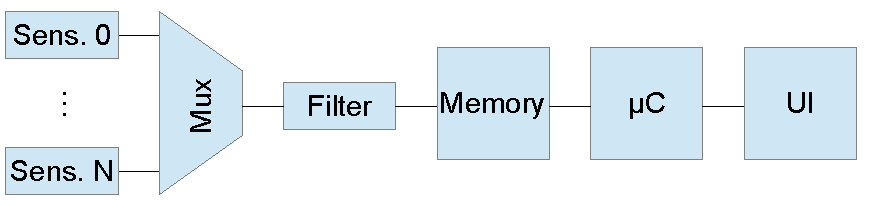
\includegraphics[scale=0.8]{global.pdf}
	\caption{Schema bloc du système}
\end{figure}


\section{Composants analogiques et échantillonage}

On peut citer beaucoup grandeurs à mesurer dans une voiture.
\begin{itemize}
\item
	Tachymètres, pour mesurer la vitesse des roues et du moteur.
\item
	Thermomètres, pour mesurer la température extérieure et du moteur.
\item
	Baromètres, pour la pression de l'huile et autres fluides.
\end{itemize}

\begin{figure}[h!]
	\centering
	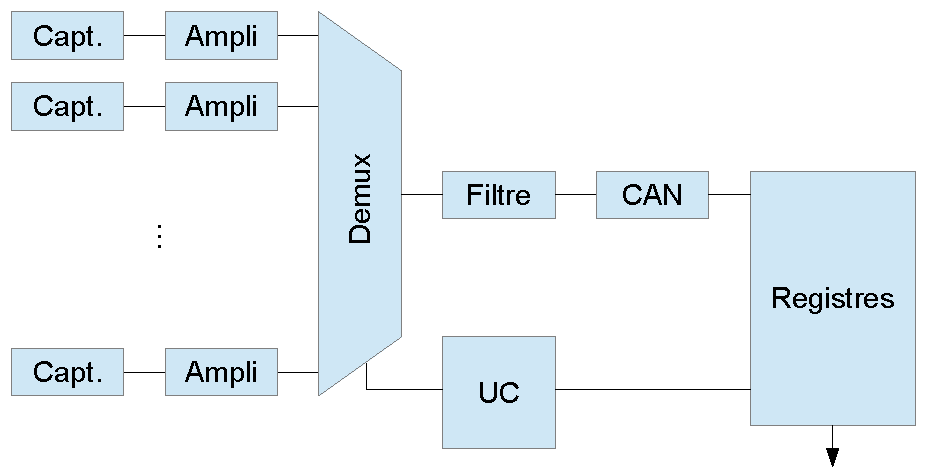
\includegraphics[scale=0.8]{sensor.pdf}
	\caption{Schéma bloc du système de mesure}
\end{figure}

Des amplificateurs sont utilisés sur les capteurs pour permettre au signal analogique de parcourir les grandes distances qui les séparent du système central.

Pour économiser le nombre de composants utilisés, on n'utilise qu'un seul convertisseur analogique-numérique, après un multiplexeur.
Un contrôleur s'occupe d'échantillonner successivement les différents capteurs, pour mettre à jour les registres qui leur correspondent.

Ces informations ne requièrent pas une précision élevée.
Nous avons donc choisi une fréquence d'échantillonage pour chaque capteur de $10 H\!z$.
Ainsi, si nous avons 5 capteurs, le contrôleur aura une fréquence de $50 H\!z$.

Après le multiplexeur, un filtre actif s'occupe de nettoyer le signal.
On a opté pour un simple filtre passe-bas, afin de filtrer les fréquences supérieures à $10 H\!z$.
Il serait bien sûr possible de cascader ce filtre pour améliorer la qualité (et éventuellement considérer d'autres types de filtres, tel le Sallen-Key de Butterworth d'ordre $N$).

L'étape suivante consiste à convertir le signal analogique en signal numérique.
Pour cela, on a à disposition plusieurs sortes de convertisseurs.
Nous avons choisi la famille de convertisseurs A/N à approximations successives, étant adaptés pour un usage général.
En effet, ils représentent un bon compromis précision, vitesse, prix.

Le seul désavantage de ce genre de convertisseur est le nombre limité de bits disponibles (8 à 14 bits).
Pour corriger ce problème, il est possible de monter ces CAN en cascade, et ainsi augmenter la résolution.
Nous estimons que 16 bits sont suffisants pour les grandeurs que nous utilisons.


\begin{figure}[h!]
	\centering
	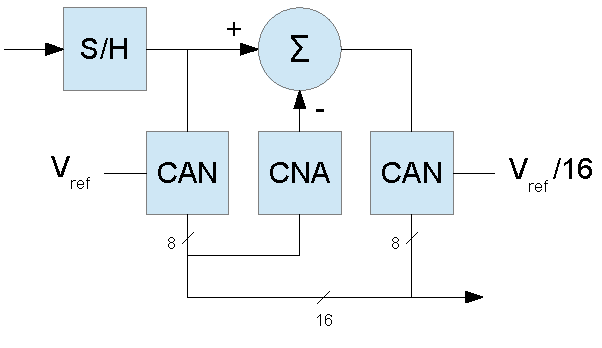
\includegraphics[scale=0.8]{can.pdf}
	\caption{Convertisseur analogique-digital 16-bits}
\end{figure}

Enfin, ce signal numérique est mémorisé dans des registres, qui pourront être lus par l'unité principale.


\section{Unités de contrôle et de traitement}

\begin{figure}[h!]
	\centering
	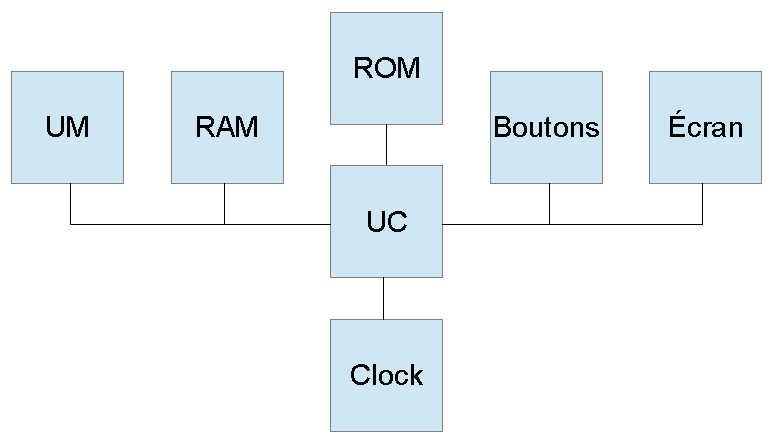
\includegraphics[scale=0.8]{uc.pdf}
	\caption{Schéma bloc du système}
\end{figure}

L'unité de contrôle (UC) est reliée à tous les autres composants, et se charge de coordonner les tâches.

Du côté de la mémoire, les différents registres des capteurs sont accessibles en lecture seule.
Une mémoire SRAM nous paraît être un bon choix, rapide et robuste.
Au vu de la taille minime nécessaire, son coût est acceptable.

À cela s'ajoute une autre mémoire vive qui contient les données nécessaires au système.
De nouveau, nous utilisons une SRAM pour conserver les valeurs (compteur kilométrique, par exemple) lorsque le système est sous tension.
Et lorsque le système est privé d'alimentation, une copie de la mémoire est sauvegardée sur une mémoire non-volatile, de type Flash.
Cette décision est motivée par le nombre limité d'écriture sur les supports Flash.
En effet, avec une fréquence d'écriture de $10 H\!z$, la mémoire Flash atteindrait rapidement ses limites de réécriture.

\begin{figure}[h!]
	\centering
	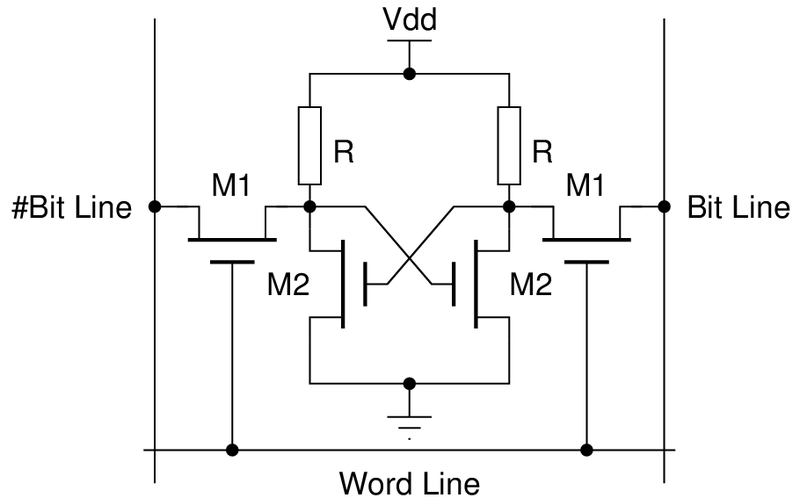
\includegraphics[scale=0.4]{4T_SRAM_Cell.png}
	\caption{SRAM (source \href{http://en.wikipedia.org/wiki/Static_random-access_memory}{Wikipédia})}
\end{figure}

\todo[inline]{UC description du fonctionnement (algorithmes?)}

\subsection{Clock}
\lstinputlisting[caption=Module de contrôle de l'horloge]{ecu_clock.vhd}

\subsection{Electronic Control Unit}

\missingfigure{Graphe des états}

\lstinputlisting[caption=Module de gestion du système (UC)]{ecu.vhd}

\section{Simulation - interface utilisateur}

\missingfigure{Java UI}

L'interface utilisateur a été implémenté en utilisant en tâche de fond \textit{ModelSim}, qui permet de simuler du code VHDL.
L'idée est d'utiliser directement le vrai code VHDL de notre interface en simulant les entrées/sorties du système de mesure.

Le module d'affichage a été développé en Java, en utilisant le framework \textit{Spring}\footnote{\url{http://www.springsource.org/}} pour simplifier le travail.
Le module de simulation est une coopération entre Java et VHDL.
En VHDL la simulation est effectuée, alors qu'en Java le traitement des données est fait.

\todo[inline]{fonctionnalités (boutons, affichage...)}

Voici un exemple de listing permettant de contrôler le simulateur.

\lstinputlisting[caption=Testbench de contrôle du Simuateur en VHDL]{simulator.vhd}


\section{Conclusion}

\todo[inline]{Just say something here -\_-}

\end{document}